\documentclass[12p]{paper}
\usepackage{amsmath}
\usepackage{amssymb}
\usepackage{authblk}
\usepackage{graphicx}

\begin{document}

\title{Characterization of Windowless Silicon Avalanche Photo-Diodes with Monoenergetic Electrons in the 90-900 eV Range}

\author[1]{Alice Apponi}
\author[1]{Gianluca Cavoto}
\author[2]{Marco Iannone}
\author[1]{Carlo Mariani}
\author[2,*]{Francesco Pandolfi}
\author[2]{Ilaria Rago}
\author[3]{Alessandro Ruocco}

\affil[2]{INFN Sezione di Roma, Rome, Italy}
\affil[1]{`Sapienza' Universit\`{a} di Roma e INFN Sezione di Roma, Rome, Italy}
\affil[3]{Universit\`a di Roma Tre e INFN Sezione di Roma Tre, Rome, Italy}
\affil[*]{Corresponding author. E-mail address: francesco.pandolfi@roma1.infn.it}

\maketitle


\abstract{We report on the characterization of the response of avalanche photo-diodes to electrons in the 90-900~eV energy range. The electrons were provided by a monoenergetic electron gun }


\newpage
\clearpage


\section{Introduction}


\begin{figure}[t]
  \centering
  \includegraphics[width=0.89\textwidth]{figures/nanouv.pdf}
 \caption{Schematic view of the NanoUV detector concept.
  \label{fig:nanouv}}
\end{figure}



The results presented in this paper were produced in the context of the development of a novel UV light detector (NanoUV), with a photocathode made of vertically-aligned carbon nanotubes. The photoelectrons, upon exiting the nanotubes, are accelerated by an applied tension $\Delta V \lesssim 1$~kV, and then detected by a silicon avalanche photo-diode (APD) placed at the other end of a vacuum tube a few centimeters long. A schematic view of the NanoUV detector concept can be seen in Figure~\ref{fig:nanouv}. 

While APDs are typically employed as photon detectors, they can also be used to detect low-energy electrons. 
Upon entering the silicon, an electron loses energy through ionization, and if its inital energy is sufficiently low, it will have a range smaller than the depth of the silicon, and therefore be absorbed inside the APD. For this reason, the number of created electron-hole pairs will be proportional to the electron energy, and so will be the resulting current generated by the APD.

\begin{figure}[htb]
  \centering
  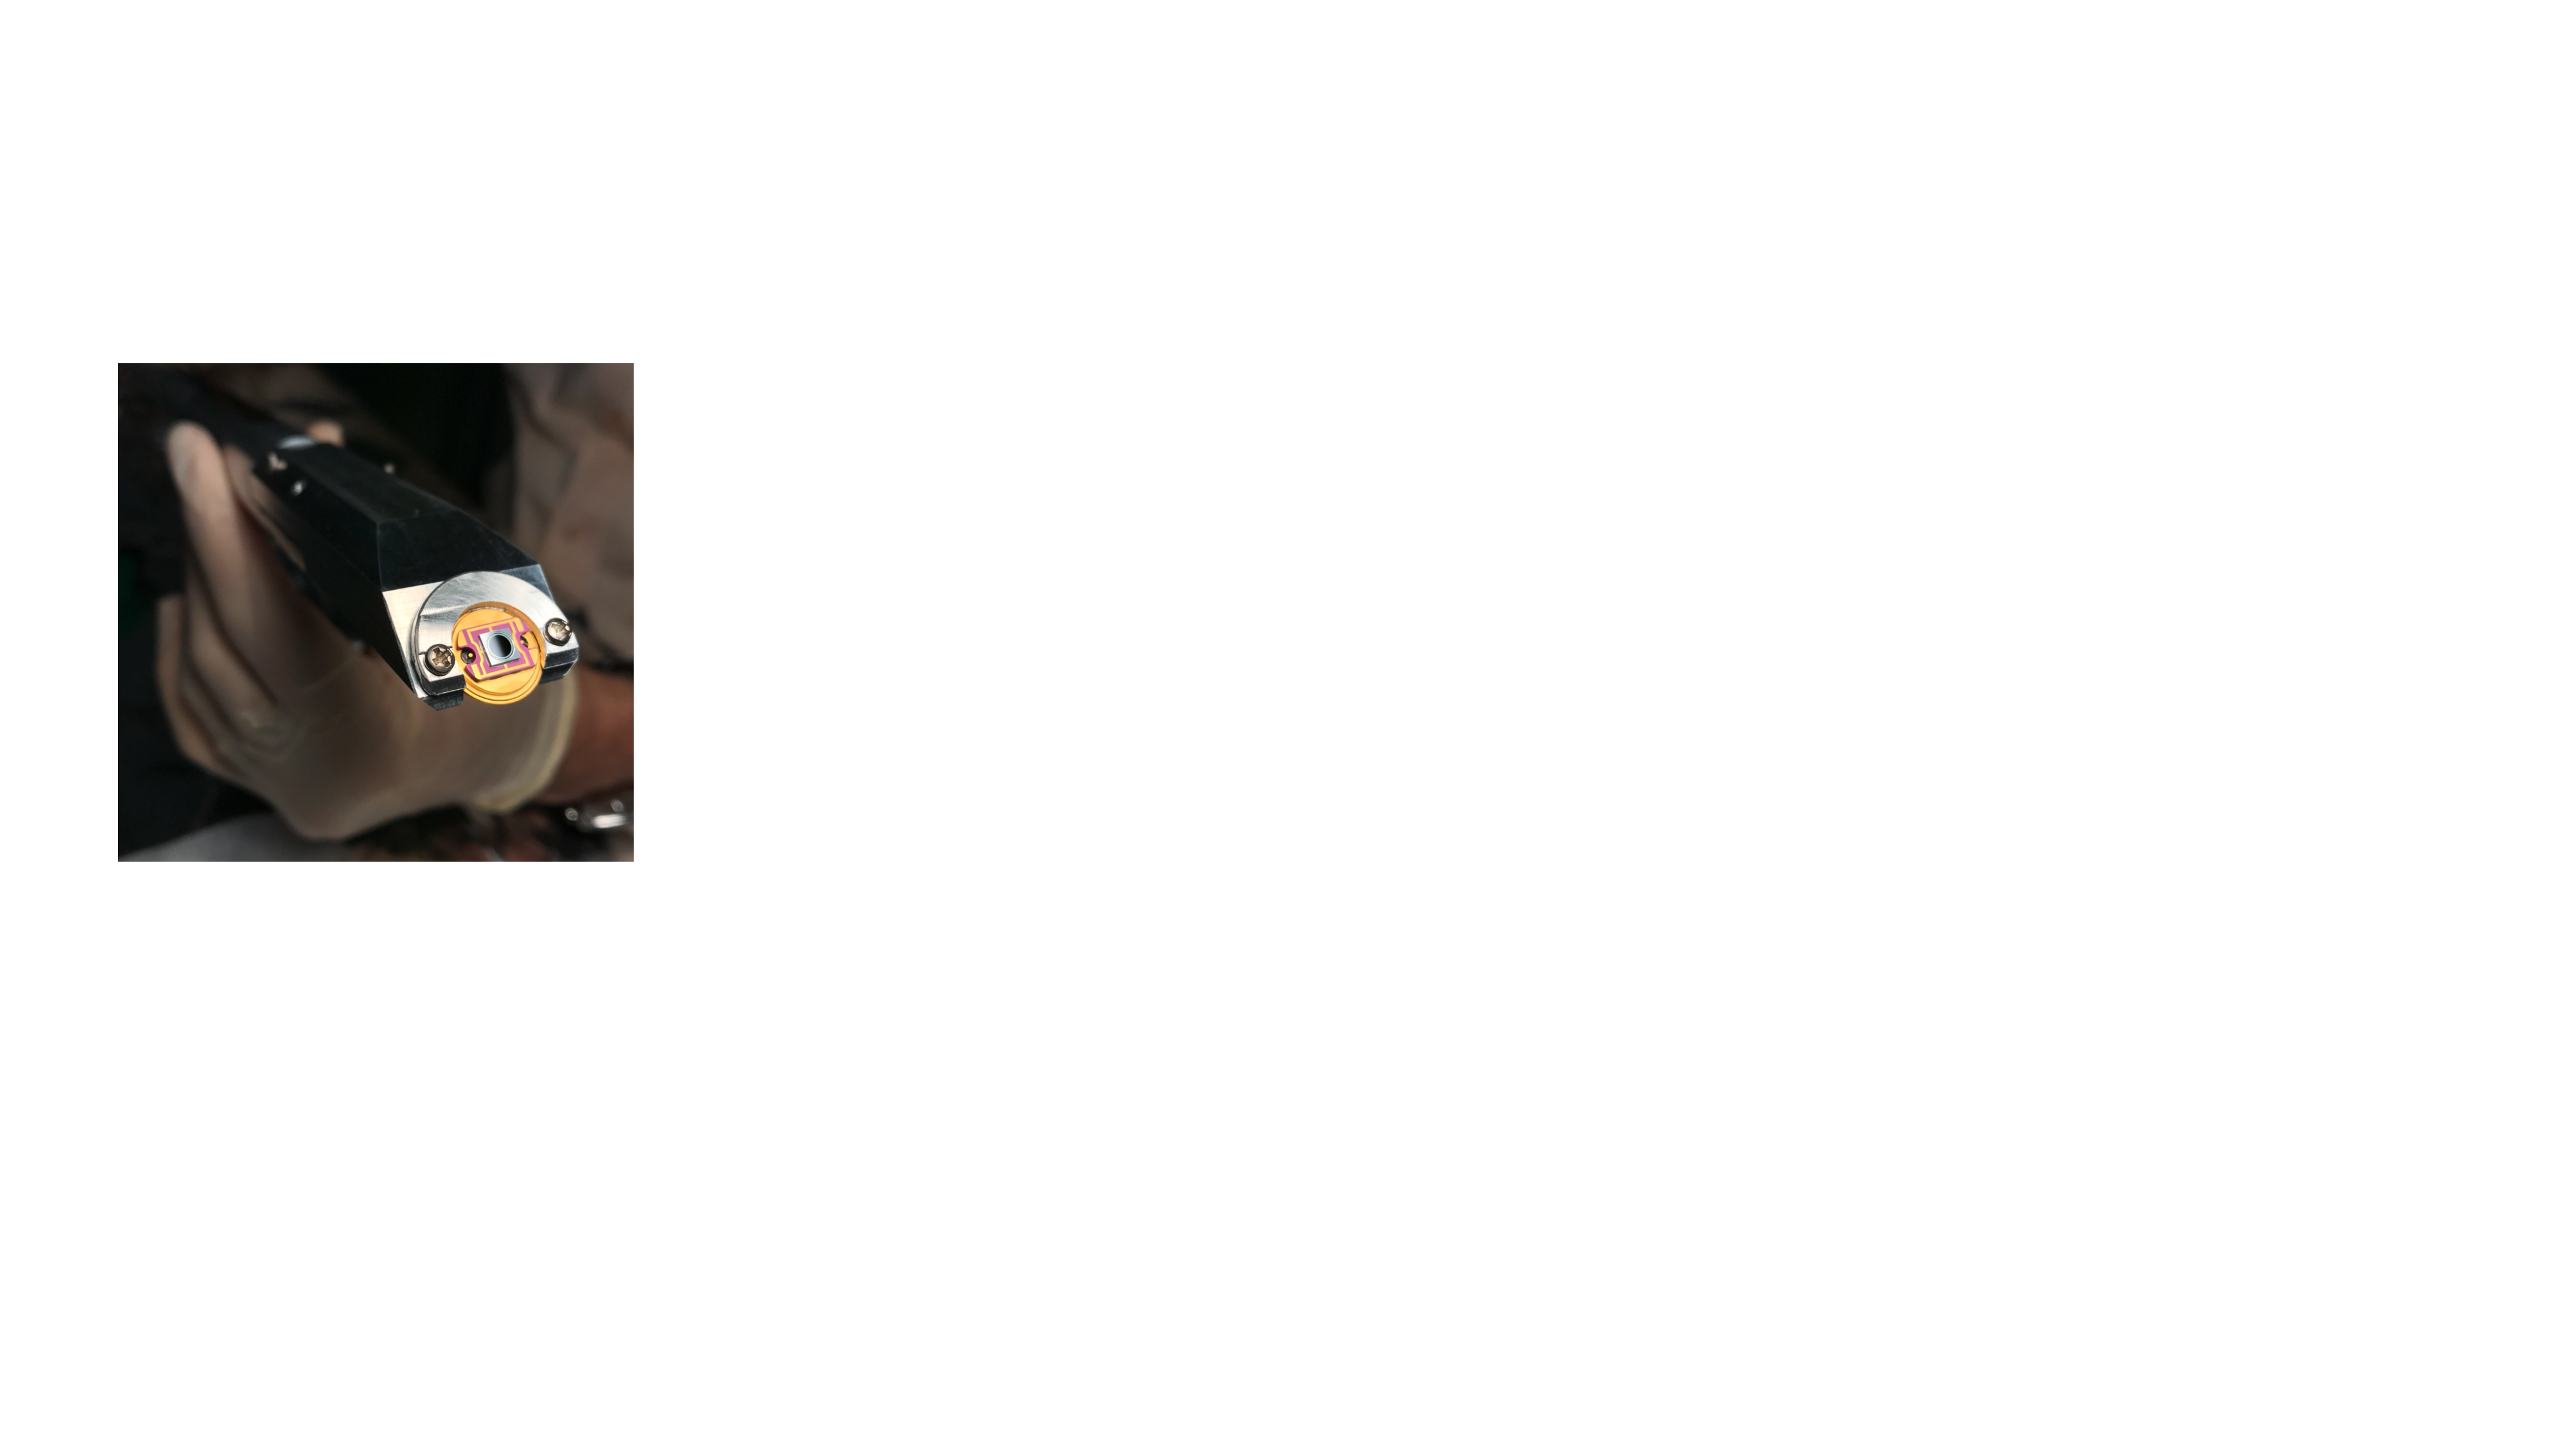
\includegraphics[width=0.59\textwidth]{figures/apd.pdf}
 \caption{Avalanche photo-diode S11625-30N by Hamamatsu Photonics mounted on the custom-made support to be inserted in the UHV chamber.
  \label{fig:apd}}
\end{figure}


\section{Experimental Apparatus}

Commercial APDs typically cover the silicon sensor with a protective layer (or `window'), which is transparent for photons, but would result in the absorption of low-energy electrons, thus compromising its performance as an electron detector. For this reason we are employing special window-less APDs manufactured by Hamamatsu Photonics (S11625-30N), which can be seen in Figure~\ref{fig:apd}. The active area is circular, and has a diameter of 3~mm. According to the factory specifications, the APD we tested is expected to have a gain $G = 50$ when operating at a bias $V_{apd} = 355.5$~V (for $\lambda = 650$~nm, at $25^{\circ}$C).

The APD is powered with a Silena 7712 power supply, at a nominal working bias of $V_{apd} = 350$~V. Throughout this paper all APD measurements are performed with a Keithley 6485 picoammeter connected to the bias pin of the APD. These are therefore measurements of the bias current of the APD, not of its output. This allows us to operate the APD even without electronics dedicated to the shaping and acquisition of its output, which is a feature which could be attractive when designing a simple light-weight detector, such as the NanoUV concept. 

\begin{figure}[tb]
  \centering
\includegraphics[width=0.69\textwidth]{figures/chamber_photo}
 \caption{Picture of the interior of the UHV chamber present in LASEC labs in University of Roma Tre: the electron gun (`e$^{-}$ source') shoots electrons towards the center of the chamber, where either the APD or the Faraday cup can be present. The UV lamp and analyzer are not used in the results presented in this paper.
  \label{fig:gun}}
\end{figure}


The APD characterization was performed in the LASEC laboratories at Roma Tre University. The APD is mounted on a custom-made support in anticorodal, and is inserted inside the UHV chamber, where is can be brought to the line of sight of the electron gun. Alternatively, when the APD is kept in its retracted position, a Faraday cup for the precise measurement of the beam current and profile can be brought in the gun focus region. A schematic view of the apparatus can be seen in Fig.~\ref{fig:gun}.

The electron gun comprises of a hot tungsten filament, followed by a system of electrostatic fields generated by spherical metal elements to select monoenergetic electrons. Additional metal plates are used to deflect the electron beam in the $x$ and $y$ directions. The gun is capable of producing beams of electrons between about 90 and 900~eV, with an energy dispersion of less than 1\%. The beam current is controlled through the Keysight B2987A picoammeter (nominal resolution: 0.01~fA), and can produce stable monoergetic electron beams down to a few~fA, which corresponds to an electron rate of $O(10$~kHz).


\section{Experimental Procedure}

\begin{figure}[tb]
  \centering
\includegraphics[width=0.99\textwidth]{figures/FC_scan.pdf}
 \caption{Measurement of the Faraday cup current (left) and its derivative (right) when sweeping the electron beam across its diameter.
  \label{fig:FC_scan}}
\end{figure}


The beam profile is measured {\em in situ} with the Faraday cup. The beam sweep is performed across the front face of the cup, along its diameter. The current of the cup is measured and a typical current profile can be seen in Fig.~\ref{fig:FC_scan}~(left), which was obtained for a beam with energy $E_e = 900$~eV and current $I_e = XXX$~pA: as can be seen the measured current is zero when the gun is shooting outside of the central hole of the cup (for $x < -7.5$~mm and $x > +4$~mm), while it is different from zero when the beam is shooting inside the cup (for $-7.5 < x < +4$~mm). 

By taking the derivative of the current profile across the cup the beam profile can be measured. This is shown in Fig.~\ref{fig:FC_scan}~(right): the resulting structures are fitted with two gaussian distributions, and the their width~$\sigma$ (which is constrained in the fit to be the same for both gaussians) is taken as a measurement of the beam profile. The result for the shown beam configuration is~$\sigma = 0.5XX$~mm, which is a typical value for all electron energies and beam currents investigated in this paper.  

\begin{figure}[tb]
  \centering
\includegraphics[width=0.49\textwidth]{figures/scanAPD.pdf}
\includegraphics[width=0.49\textwidth]{figures/scanAPD_corr.pdf}
 \caption{Measurement of the APD current when sweeping the electron beam across its sensitive area, along its diameter, before~(left) and after~(right) the dark current subtraction.
  \label{fig:apd_scan}}
\end{figure}

A similar technique is used to measure the response of the APD. A beam sweep is performed across the sensitive area of the photo-diode, and the current generated by the APD is recorded. A typical scan is shown in Figure~\ref{fig:apd_scan}~(left): as can be seen the APD generates a non-zero (dark) current even when the gun is directed outside of the silicon. As soon as the gun enters the sensitive area of the diode, the measured current increases. As can be seen, the region in which this happens has an extension of about 3~mm, which coincides with the diameter of the Hamamatsu photo-diode.

To have a precise estimate of the current generated in the APD by the gun electrons, we subtract the contribution of the dark current. This is done by fitting the first 12 and last 12 points of the scan, which are sufficiently far from the sensitive region, with a third-degree polynomial function. The choice of a non-constant function is motivated by the possibility that the diode might heat up during a scan (which takes a few minutes), and therefore induce a drift in the dark current. The dark current contribution is then subtracted, and the resulting background-subtracted scan is shown in Figure~\ref{fig:apd_scan}~(right).

\begin{figure}[tb]
  \centering
\includegraphics[width=0.49\textwidth]{figures/apdSyst.pdf}
 \caption{Example of empty APD scan used for the estimation of the systematic uncertainty connected with the fitting procedure. The open markers indicate the points used in the fit, and the red line the result of the polynomial fit. The fit result is compared to the markers in the central region of the scan (solid black) to evaluate the goodness of the extrapolation.
  \label{fig:apd_syst}}
\end{figure}

Possible systematic uncertainties on the dark-current fitting method have been estimated by taking `empty' scans, i.e. scans in which the gun was never directed over the sensitive region of the APD. An example of such scan is shown in Figure~\ref{fig:apd_syst}, where one can see the APD dark current drifting during the course of the scan. The same fitting procedure is then applied to the empty scan, by fitting the first and last 12 points of the scan (open markers in the figure), and then the fitted function is compared to the measured points in the rest of the scan (solid markers). The difference between prediction and measurement has an average compatible with zero, indicating that there is no bias in the procedure, while its width is found to be 1.22~pA, so this value is taken as systematic uncertainty on the dark-current subtraction method. 

\begin{figure}[p]
  \centering
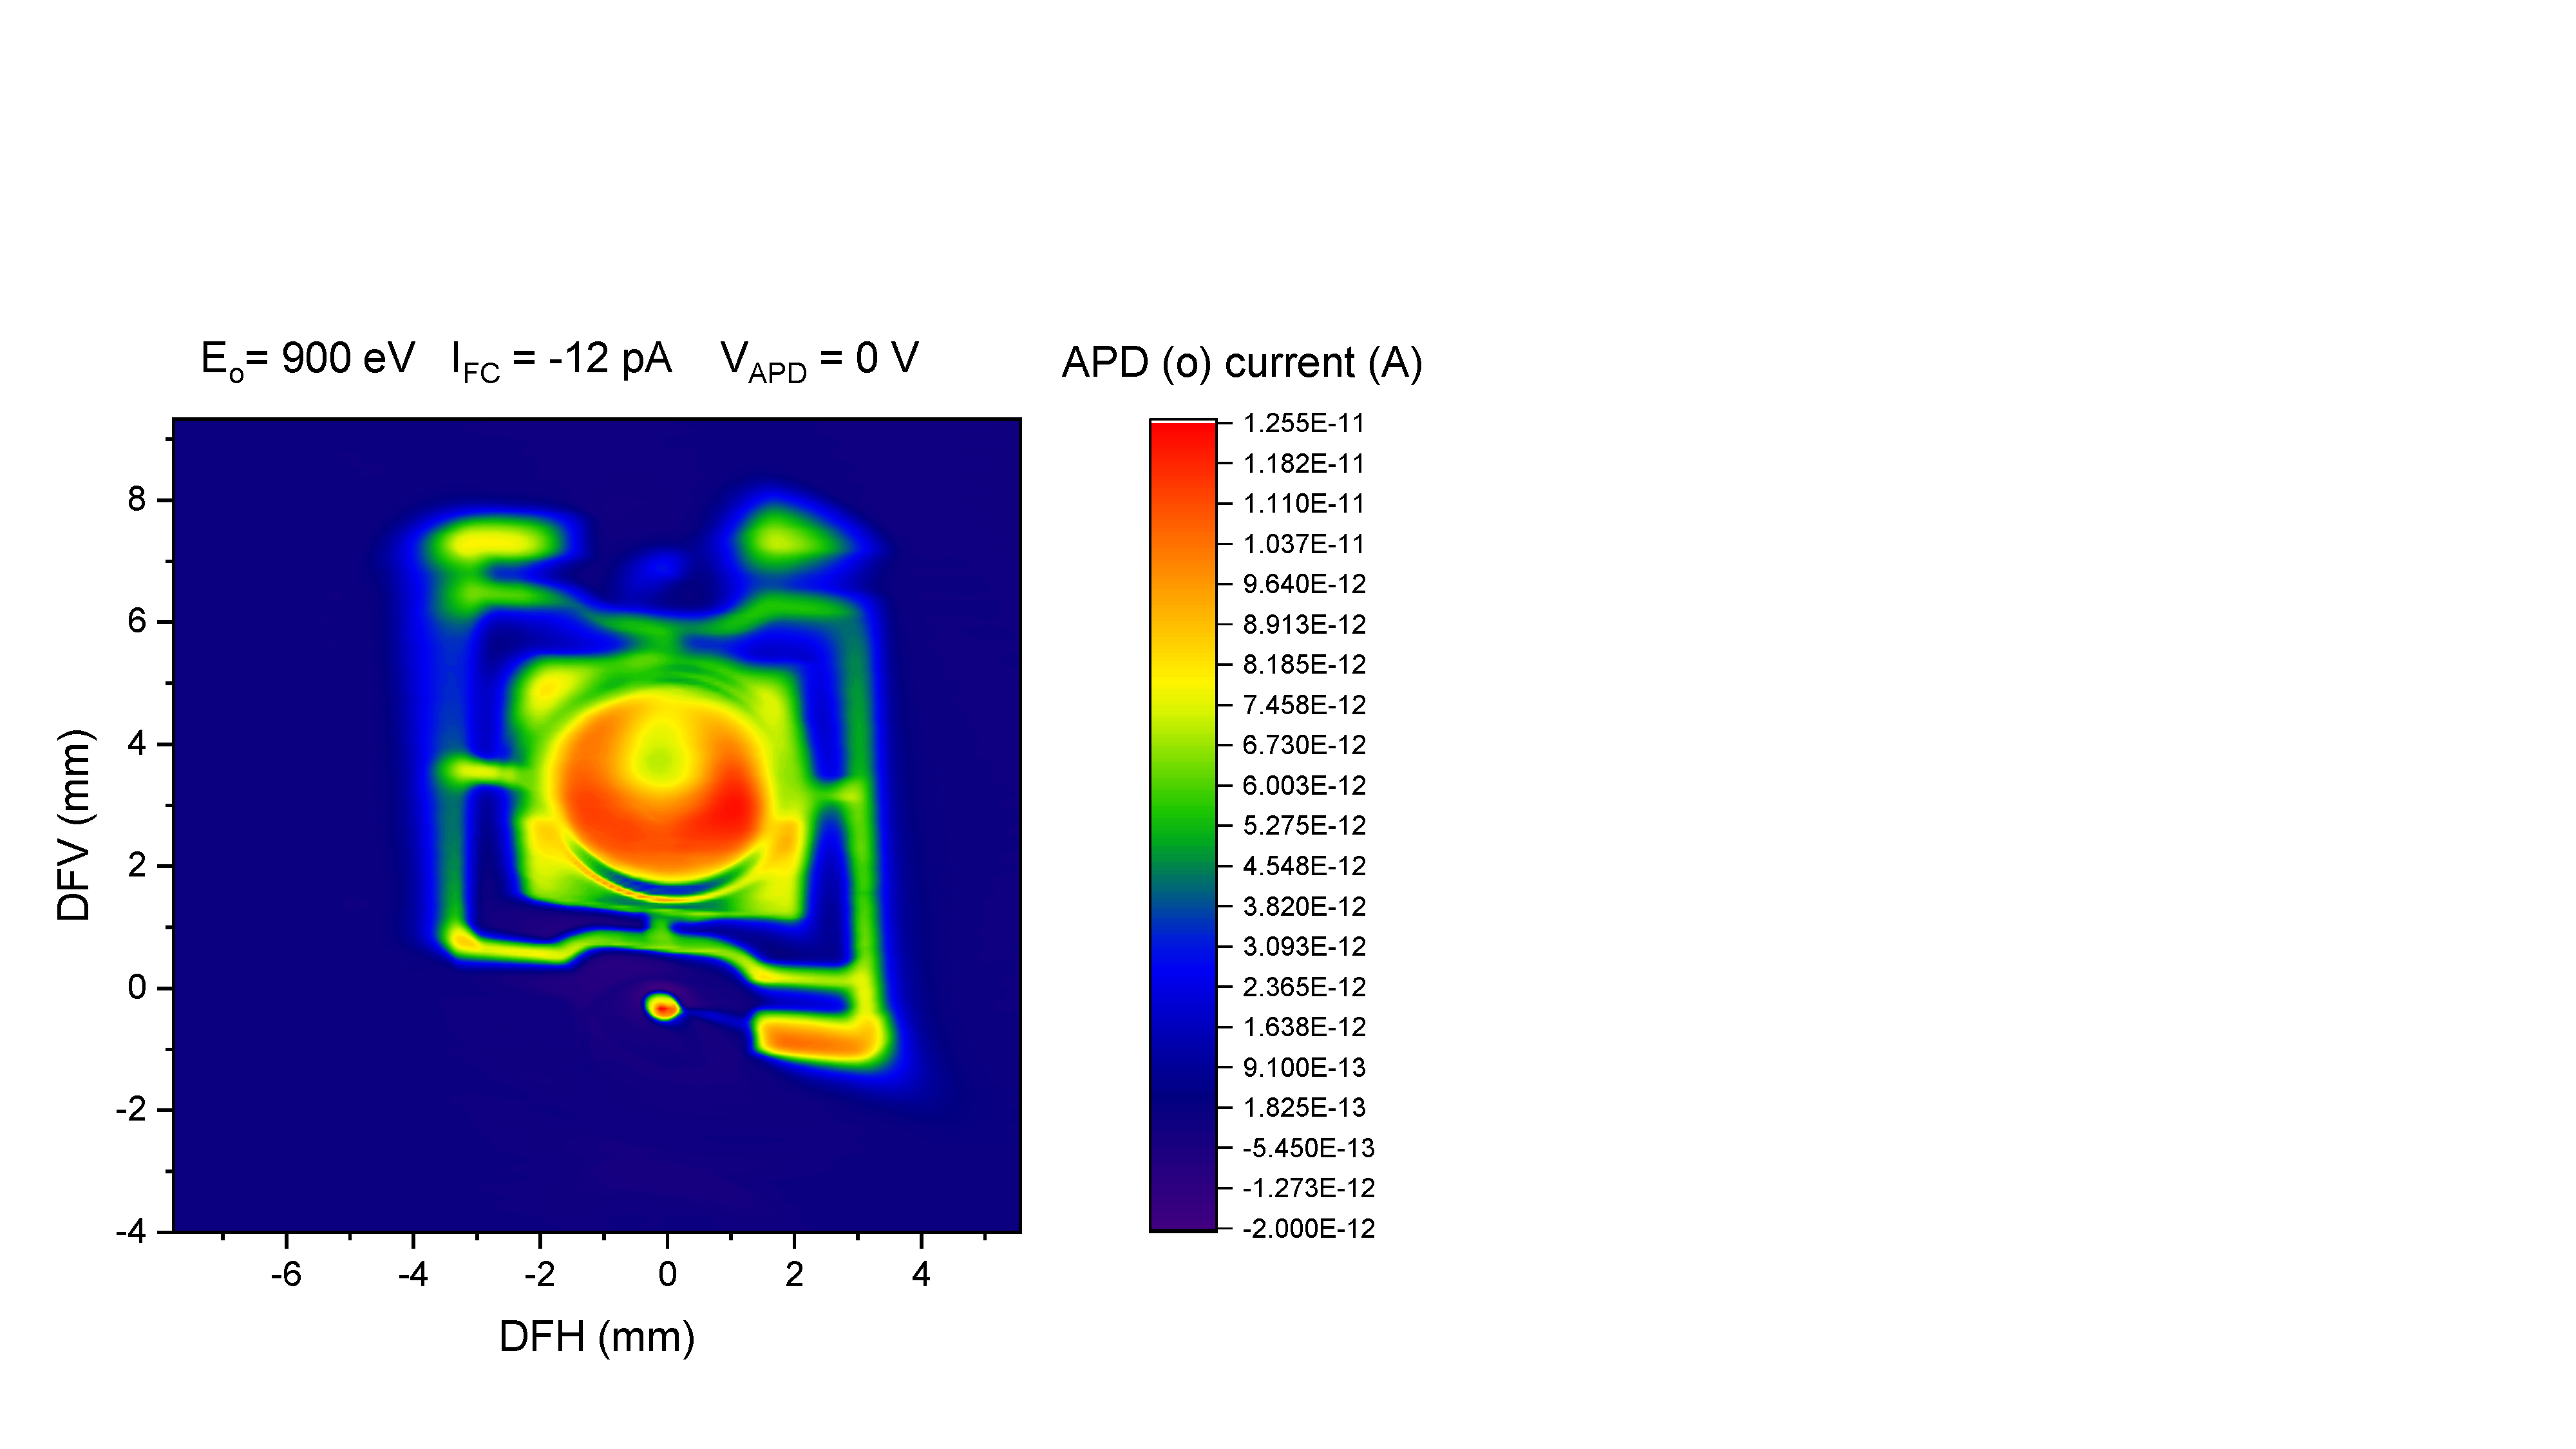
\includegraphics[width=0.61\textwidth]{figures/APD_scan_V0}
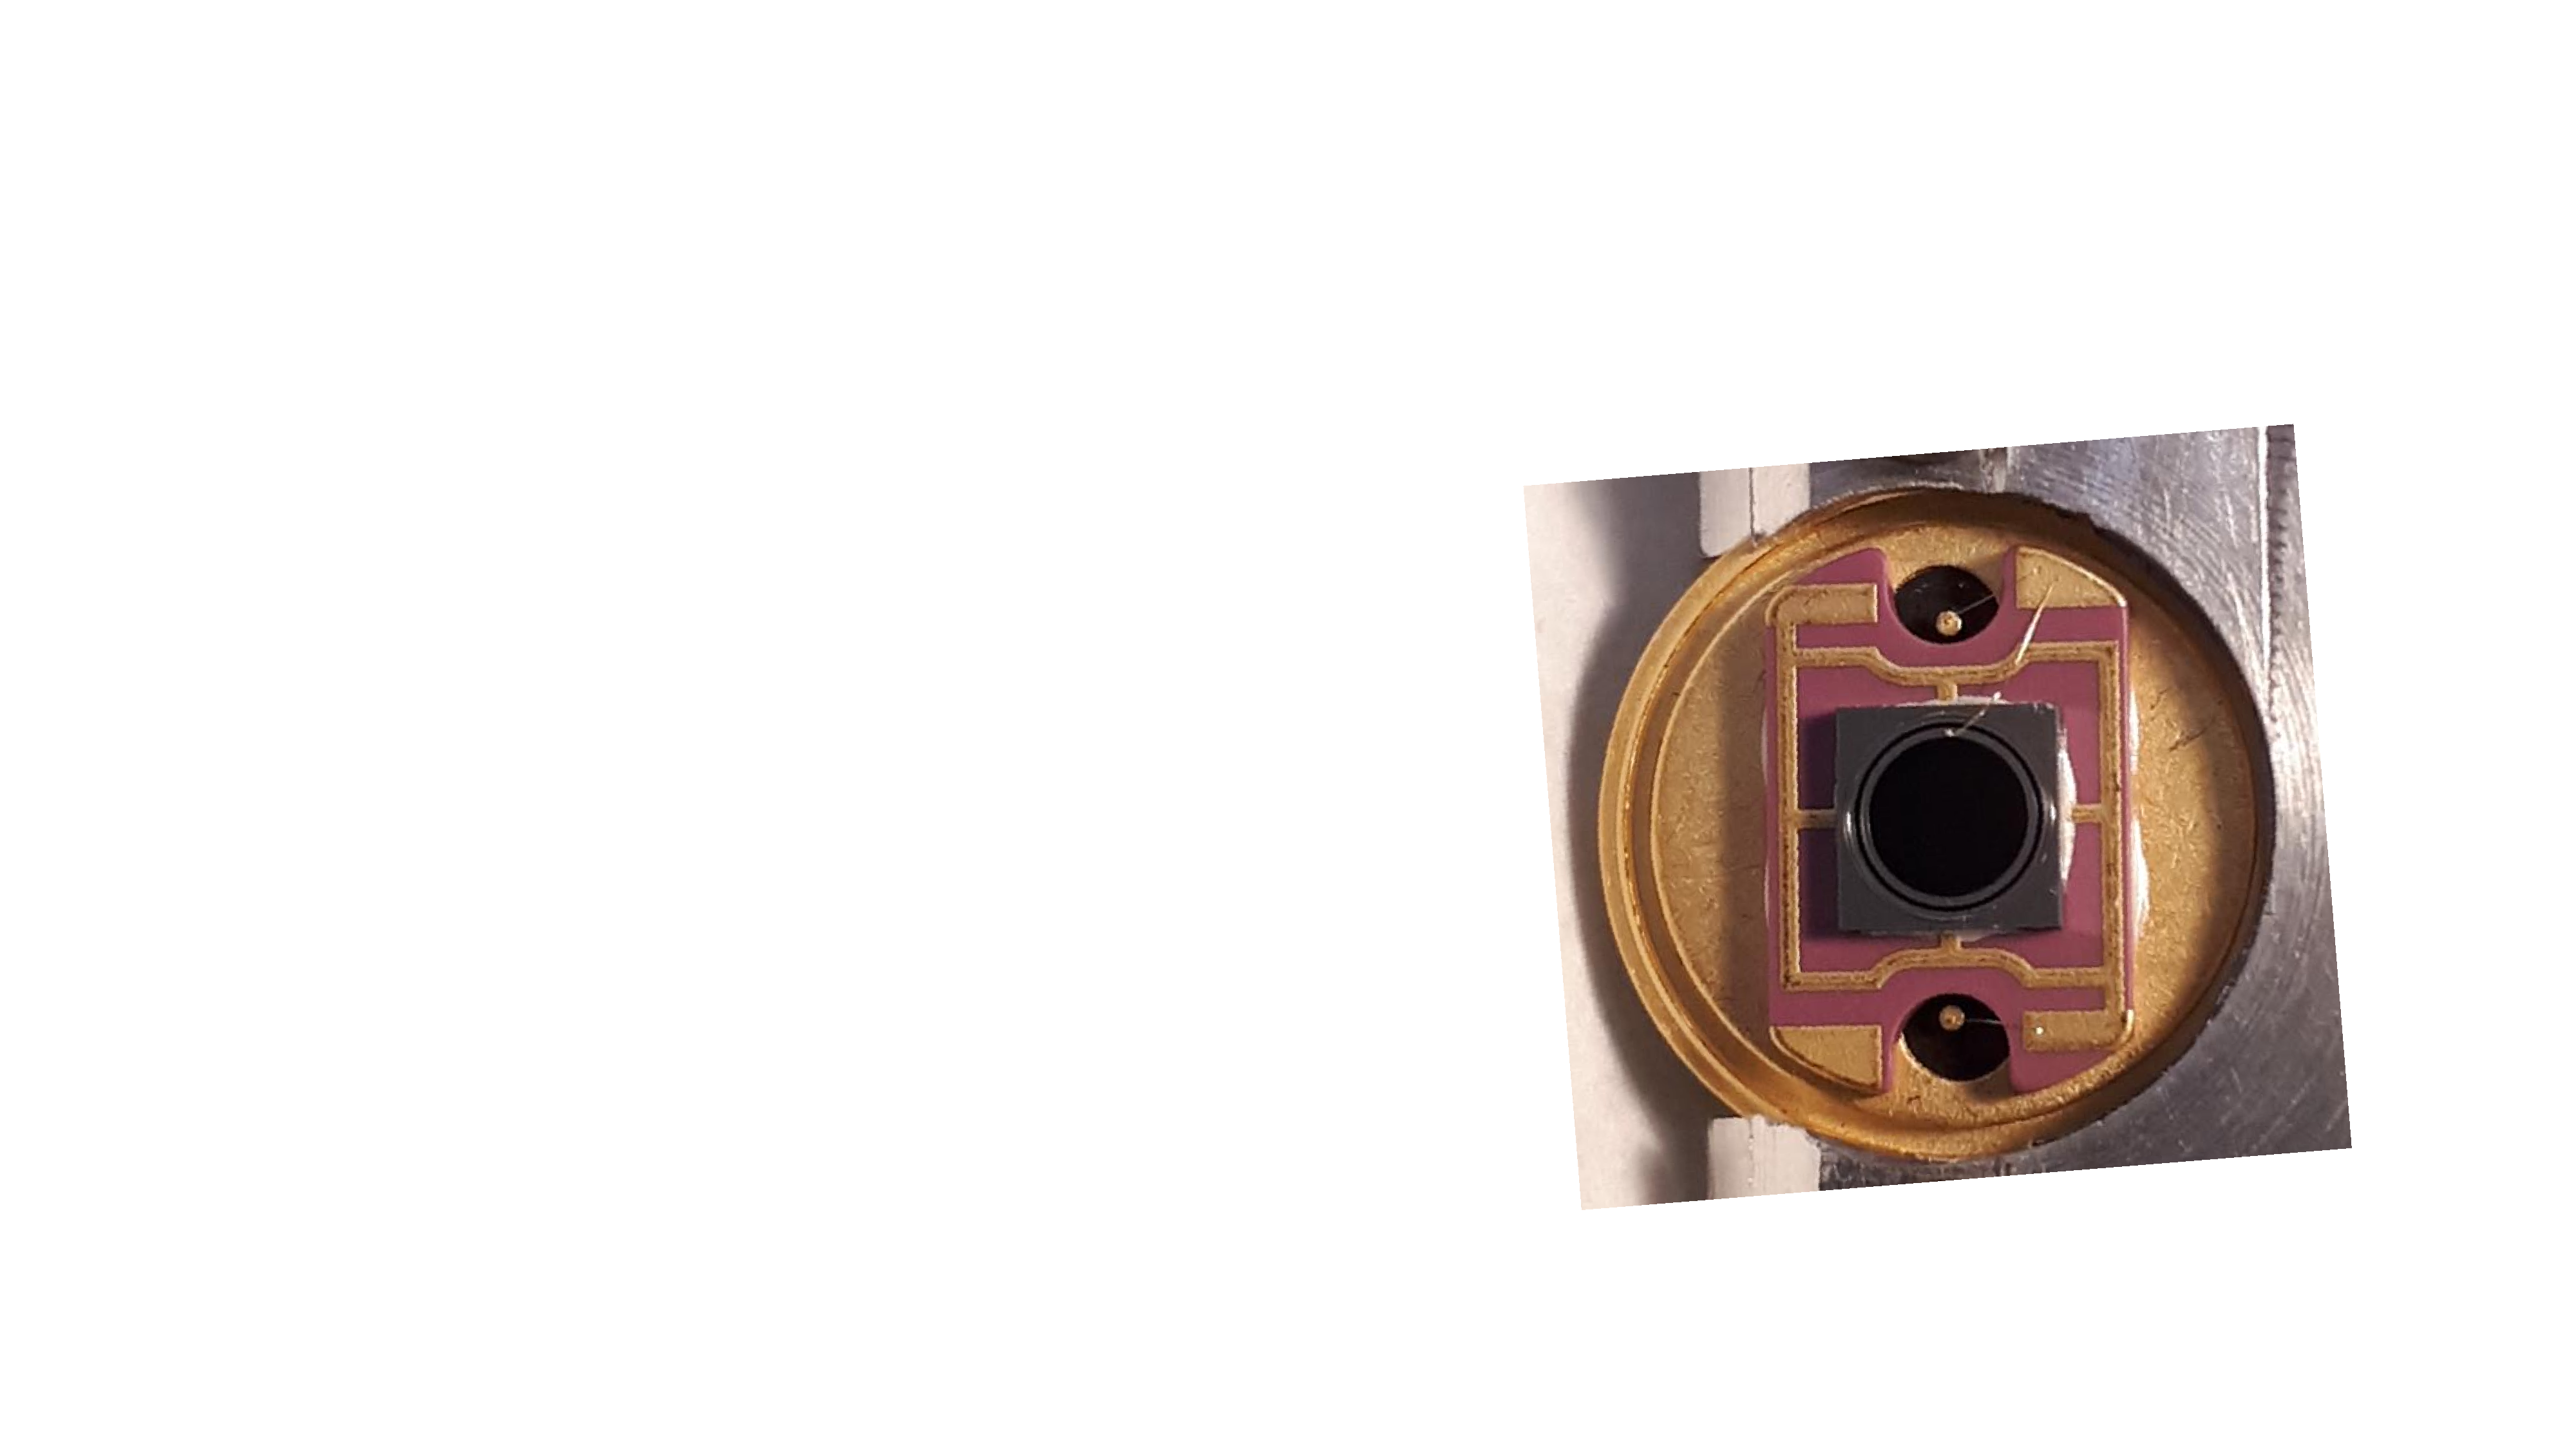
\includegraphics[width=0.38\textwidth]{figures/APD_pic}
 \caption{Measurement of the APD current as a function of the electron beam position, when sweeping the electron beam across the full front face of the APD, for $V_{apd} = 0$~V. The left plot shows the result of the scan, while a photo of the APD is shown on the right.
  \label{fig:2d_scan_V0}}
\end{figure}
\begin{figure}[p]
  \centering
\includegraphics[width=0.49\textwidth]{figures/APD_scan_V350}
\includegraphics[width=0.49\textwidth]{figures/APD_scan_V350_3d}
 \caption{Measurement of the APD current as a function of the electron beam position, when sweeping the electron beam across the full front face of the APD, for $V_{apd} = 350$~V. The left (right) plot shows a 2-dimensional (3-dimensional) view of the scan.
  \label{fig:2d_scan_V350}}
\end{figure}

By proceding in a similar fashion, we also performed 2-dimensional scans, directing the electron beam across the whole surface of the APD. This is shown in Figure~\ref{fig:2d_scan_V0} (left), where the measured APD current is shown on the $z$-axis, as a function of the $x-y$ position of the incident electron beam. This scan was produced keeping the APD unpolarized ($V_{apd} = 0$~V). As can be seen, our apparatus is sensitive to very small fluctuations in the bias current, so the resulting `image' created with the electron beam, reproduces in great detail the APD structure (shown in the figure on the right, as reference), down to all of the metal contacts. As can be seen, the left image is sharpest in correspondence of the origin ($x=y=0$), and gradually worsens its resolution when moving away. This is due to beam defocusing effects, which are minimal when the beam is not deflected.

A similar 2-dimensional scan was performed while operating the APD at the nominal bias $V_{apd}=350$~V, and the results are shown in Figure~\ref{fig:2d_scan_V350}, where the right plot is simply a 3-dimensional rendering of the left one. As can be seen, when increasing the APD bias, the response of the sensitive region of the silicon is greatly enhanced. Furthermore, we observe a small region towards the upper part of the detector where we observe a dip in the response of about a factor two. Because of this we have excluded that region from subsequent studies, by performing linear scans across the equatorial diameter of the APD (horizontally, at $y\sim 3$ mm).
\clearpage

\section{Results}

To measure the APD response to the gun current, we perform equatorial beam sweeps for multiple gun currents in the range $0.1 \div 10$~pA. To check the current stability, for each gun current setting the gun current is measured with the Faraday cup before and after the APD sweep. The uncertainty on the gun current is taken as either half of the absolute difference between these two measurements, or 0.5\% of their average value, whichever is largest.

The APD current is extracted from the sweep profiles. Once the dark-current contribution is subtracted as described in the previous section, the maximum current is identified, and only points which have a current larger than 50\% of the maximum are considered. The APD current $I_{apd}$ is taken as the average of these points. The uncertainty on $I_{apd}$ is taken by propagating to the average a single-point uncertainty, which in turn is taken as the quadrature sum of the resolution (0.1~pA) plus the systematic uncertainty on the background subtraction (1.22~pA).

We have estimated the systematic uncertainty connected to the choice of this definition of $I_{apd}$ by computing, in each point, an alternative current estimator. This alternative estimator defines $I_{apd}$ by first computing the integral of the background-subtracted scan, and then dividing the result by the APD nominal diameter~(3~mm). The two $I_{apd}$ definitions are found to be in good agreement,  except for the integral method giving values systematically 10\% larger than the nominal method, because of its complete inclusion of the tails. After taking into account this constant scale factor, we take residual differences between the two methods as a systematic uncertainty: this uncertainty is found to be no larger than a few percent for all measured points, except for the lowest $I_{gun}$ values of $E_e = 500$~eV, where it rises to up to 25\%. 

\begin{figure}[htb]
  \centering
  \includegraphics[width=0.49\textwidth]{figures/iapd_vs_igun_E500_V350}
  \includegraphics[width=0.49\textwidth]{figures/iapd_vs_igun_E900_V350}
 \caption{APD current as a function of the electron gun current, for $E_{e} = 500$~eV (left) and $E_{e} = 900$~eV(right).
  \label{fig:i_vs_i}}
\end{figure}

The results are shown in Figure~\ref{fig:i_vs_i}: the left plot corresponds to $E_{e} = 500$~eV, the right one to $E_{e} = 900$~eV. As can be seen a linear dependence between $I_{apd}$ and $I_{gun}$ is observed, and the trends have been fitted with the function:
$$
I_{apd} = I_0 + G\cdot I_{gun},
$$
shown with a dashed red line in the plots. As can be seen the linear hypothesis seems to be supported by the data, and in both cases the intercept $I_0$ is found to be compartible with zero. The fitted values of $G$ are taken as measurements of the APD gain, and are summarized in Figure~\ref{fig:G_vs_E}, as a function of the electron energy. As can be seen XXX

%\begin{table}[tb]
%\centering
%\caption{Summary of the measurements of the APD gain $G$.
%\label{tab:i_vs_i}}
%\begin{tabular}{lcc}
%\hline
%& $E_{e} = 500$~eV & $E_{e} = 900$~eV \\
%$V_{apd} = 350$~V & XX & XX \\
%$V_{apd} = 380$~V & XX & XX \\
%\hline
%\end{tabular}
%\end{table}

\section{Conclusions}

\section*{Acknowledgements}

This project has received funding from the ATTRACT project funded by the EC under Grant Agreement 777222.

\end{document}